% Revised manuscript body based on the strict real-run results completed in September 2026.
% Intended to replace the scientific content of the earlier deception-llms workshop draft.
% No Mistral/Qwen headline claims are retained because those reference runs were not repeated
% under the strict real-run protocol.

\title{Poker Bluff Judgements in Llama-3.1-8B: Decodability, Confounds, and Controlled Interventions}
\author{Anonymous Authors}
\date{}
\maketitle

\begin{abstract}
We study what internal activations of Llama-3.1-8B reveal about an operationalized poker bluff label. Each example describes a no-limit Texas Hold'em state and an observed raise that has already occurred, so our task is analysis of the model's \emph{bluff judgement}, not detection of a private intention while the model chooses an action. Using 44,631 GPT-4o-labelled examples, we extract pre-response residual-stream states at the final prompt token and train layerwise logistic probes with group-safe splits and validation-only layer selection. Bluff labels are strongly decodable in both an explicit judgement prompt and a question-stripped neutral-state prompt, reaching held-out AUROC 0.936 and 0.935, respectively. However, poker-state variables are themselves highly predictive: a nuisance-only baseline reaches AUROC 0.920, and residualizing hidden states with respect to observed nuisance variables reduces the primary probe AUROC from 0.936 to 0.722. Controlled inference-time interventions along the learned probe direction produce signed, dose-dependent changes in the model's forced-choice bluff judgement, but matched random, shuffled-label, and nuisance directions can also produce substantial effects, limiting claims of direction specificity. An unsupervised TopK sparse autoencoder reconstructs the selected-layer activations well, with 95.2\% test variance explained, but individual label-associated features are weak and unstable across seeds. These results show robust late-layer encoding of the bluff label while also demonstrating that much of the apparent signal is entangled with ordinary poker strategy and that causal specificity requires stronger evidence than decodability alone.
\end{abstract}

\section{Introduction}
Internal activations provide a data source complementary to generated text. A model can encode information that is not obvious from its final output, but high probe accuracy alone does not identify what that information represents, whether it is specific to a target concept, or whether it plays a causal role in the model's behavior. These distinctions are especially important in studies of deception, where task labels can be correlated with ordinary semantic or strategic variables.

We study these issues in a constrained poker setting. Each example describes a no-limit Texas Hold'em state and includes an observed player action, specifically a raise. A separate GPT-4o labelling procedure assigns a binary bluff or non-bluff judgement. We then run Llama-3.1-8B on the resulting description and analyze the model's hidden states before it generates an answer. Because the subject model evaluates an action that has already occurred, our experiments concern representations associated with \emph{bluff judgement}. They do not establish that the model itself intends to deceive or chooses to bluff.

Poker is useful precisely because it also exposes a major interpretability confound. Bluff labels are strongly related to ordinary game-state information such as made-hand strength, street, position, and board texture. A hidden-state probe can therefore achieve high performance without isolating a distinct ``deception representation.'' We make this confound part of the experimental design rather than treating it as a caveat after the fact.

Our study asks four questions. First, how linearly decodable is the bluff label across transformer depth when activations are extracted before the answer token? Second, does removing the explicit question ``Is this a bluff?'' materially change decodability? Third, how much of probe performance survives controls for poker-state nuisance variables? Fourth, do controlled interventions along a probe-derived direction produce a specific change in the model's own bluff judgement relative to matched control directions?

Our main findings are:
\begin{itemize}
    \item Bluff labels are strongly decodable in late Llama-3.1-8B layers. The explicit judgement prompt reaches test AUROC 0.936 at physical layer 30, while the question-stripped neutral-state variant reaches 0.935 at layer 31.
    \item Removing the explicit bluff question barely changes held-out probe performance, so the headline decodability result is not explained by that wording alone.
    \item Poker-state metadata is nearly as predictive as the hidden-state probe. A nuisance-only baseline reaches AUROC 0.920, and residualizing observed nuisance information reduces the primary hidden-state probe from AUROC 0.936 to 0.722.
    \item Probe-direction interventions produce a signed dose response on the model's forced-choice bluff judgement, but several control directions also produce substantial effects. The result supports causal modulation of the judgement endpoint under intervention, not a uniquely identified bluff or deception mechanism.
    \item A 32,768-feature TopK sparse autoencoder reconstructs the selected-layer activations well but exhibits low dictionary stability across seeds and only modest single-feature label separability, arguing against strong feature-level semantic claims.
\end{itemize}

The contribution is therefore narrower than a claim of a universal deception circuit. We provide a strict case study of how high activation-level decodability can coexist with strong task confounds, how instruction wording can be tested directly, and how causal interventions should be interpreted when matched controls produce comparable effects.

\section{Task, Data, and Experimental Protocol}
\subsection{Poker bluff-judgement dataset}
The analyzed dataset contains 44,631 poker examples, with 7,490 positive bluff labels and 37,141 non-bluff labels, for a 16.8\% positive rate. Each row describes a 6-max no-limit Texas Hold'em state with player position, private cards, public board cards, betting history, and an observed raise. The bluff label is a GPT-4o yes/no judgement produced by a recovered poker-analysis prompt. The labels should therefore be interpreted as model-generated annotations rather than game-theoretic proofs or measurements of the Llama subject model's intention.

The source examples are attributable to PokerBench, but exact upstream lineage is incomplete. The exact PokerBench split or revision, original hand/session identifiers, final 44,631-row construction script, upstream action-generation procedure, and exact served GPT-4o snapshot are not recoverable from the repository history. We therefore use statement-derived grouping to prevent exact and near-identical statements from crossing partitions, but we do not describe these groups as verified independent dealt hands or sessions.

Two prompt variants are analyzed. The \texttt{judge\_question} variant retains the explicit bluff judgement wording and ends immediately before answer generation. The \texttt{neutral\_state} variant removes the target question and presents the same poker state and observed action without asking whether it is a bluff. This comparison directly measures whether the explicit target instruction is necessary for the probe result.

\subsection{Fixed group-safe split}
The strict experiments use one frozen group-safe, label-stratified split shared by all downstream analyses: 31,241 training rows, 4,463 validation rows, and 8,927 test rows. Layer selection and feature selection use training and validation data only. The test set is evaluated only after those choices are frozen. Dataset and split checksums are stored in the run artifacts, and downstream commands refuse stale or mismatched manifests.

\subsection{Activation extraction}
We use \texttt{meta-llama/Llama-3.1-8B-Instruct} at pinned model and tokenizer revision \texttt{0e9e39f2\allowbreak 49a1697\allowbreak 6918f6564\allowbreak b8830bc8\allowbreak 94c89659}, with bfloat16 weights. For every example we record the residual-stream state at the output of each of the 32 transformer blocks, using the final prompt token before the model's answer. The response label token is never provided to the extractor. The resulting activation tensor has shape 32 by 4096 for each example.

For the explicit judgement variant, extraction occurs at the prompt boundary immediately after the answer cue. For the neutral variant, extraction occurs at the end of the state-action description. The extraction manifest stores the rendered-prompt hash, token index, physical layer mapping, tensor artifact hash, model revision, tokenizer revision, and activation shape for every sample.

\subsection{Layerwise probes and baselines}
At physical transformer layer $\ell$, we fit a logistic probe
\[
    p(y=1\mid h_\ell)=\sigma(w_\ell^\top h_\ell+b_\ell),
\]
where $h_\ell$ is the final-prompt-token residual-stream state and $y=1$ denotes the GPT-4o bluff label. Probe regularization is fixed at $C=1.0$. We repeat the layerwise experiment across five seeds, select the best layer by validation AUROC only, and evaluate the frozen layer once on the held-out test set. We report AUROC, PR-AUC, calibration metrics, seed variability, and grouped bootstrap confidence intervals.

We compare the hidden-state probe against four baselines: majority-class accuracy, prompt-text TF-IDF, response-text TF-IDF as a leakage diagnostic, and a nuisance-only model using parsed poker metadata. The response-text diagnostic is expected to be perfect because the response field is the label verbatim; it is included only to make the leakage failure mode explicit.

\subsection{Learning curves}
To measure data scaling without reusing individual rows from the same statement-derived group, we train at 500, 2,000, 8,000, 20,000, and 31,000 training groups. Each size uses five independent group-level subsamples and is evaluated on the same frozen test partition at the validation-selected physical layer.

\subsection{Poker-state confound controls}
We parse nuisance variables including street, position, made-hand category, board texture, board pairing, and amount faced. We evaluate three complementary controls. First, a nuisance-only baseline estimates how predictable the bluff label is from game-state metadata alone. Second, matched-subset probes evaluate hidden-state performance within strata that equalize selected nuisance variables. Third, train-fitted residualization removes linear nuisance-predictable components from the hidden states before refitting the bluff probe.

Some desirable controls cannot be run because the required metadata is unavailable. In particular, true hand equity is not present, and reliable pot size cannot be reconstructed from the available text. The corresponding equity-matched and bet-size-matched controls are therefore reported as not run rather than approximated with unsupported quantities.

\subsection{Controlled inference-time interventions}
For the explicit judgement variant, we fit a probe-derived direction on the training partition and intervene inside the live Llama model at the validation-selected physical layer. The primary endpoint is the model's own forced-choice output distribution over the tokens `` Yes'' and `` No'', not the probe score. The held-out intervention subset contains 500 test examples sampled with group awareness.

For a hidden state $h$ and unit-norm direction $d$, steering uses
\[
    h' = h + \alpha d,
\]
with strengths $\alpha\in\{0.5,1,2,4\}$. We evaluate both signs of the learned direction and compare them against matched-norm random, orthogonal, shuffled-label, wrong-layer, wrong-token-position, mismatched-prompt activation-patching, and made-hand nuisance directions. Every effect is paired within prompt and summarized with grouped bootstrap confidence intervals. We also track probability mass on the allowed Yes/No options so that generic output degradation cannot be mistaken for a targeted effect.

\subsection{Sparse autoencoder}
We train an unsupervised TopK sparse autoencoder at the validation-selected explicit-judgement layer. The SAE has 32,768 features, an 8x expansion over the 4,096-dimensional residual stream, and exactly 64 active features per example. Training uses 60 epochs, batch size 1,024, learning rate $3\times10^{-4}$, train-only input normalization, unit-norm decoder columns, and no label information. The dictionary is frozen before held-out evaluation.

We report reconstruction mean-squared error, fraction of variance explained, mean L0, dead-feature fraction, activation frequency, and dictionary stability across three additional training seeds. Feature ranking uses train plus validation data only; selected features are evaluated once on test.

\section{Results}
\subsection{Bluff labels are strongly decodable in late layers}
The explicit judgement prompt selects physical layer 30 in all five probe runs. Validation AUROC is 0.9413 and held-out test AUROC is 0.9360. The neutral-state prompt, which removes the explicit bluff question, selects physical layer 31 in all five runs and reaches validation AUROC 0.9402 and test AUROC 0.9351.

The near-equality of these two results is important. Removing the question ``Is this a bluff?'' changes test AUROC by less than 0.001. Thus, the strong linear signal does not depend on the subject model being explicitly instructed to classify bluffing. At the same time, this comparison does not by itself establish a bluff-specific representation, because the underlying game state remains strongly correlated with the label.

\begin{figure}[t]
\centering
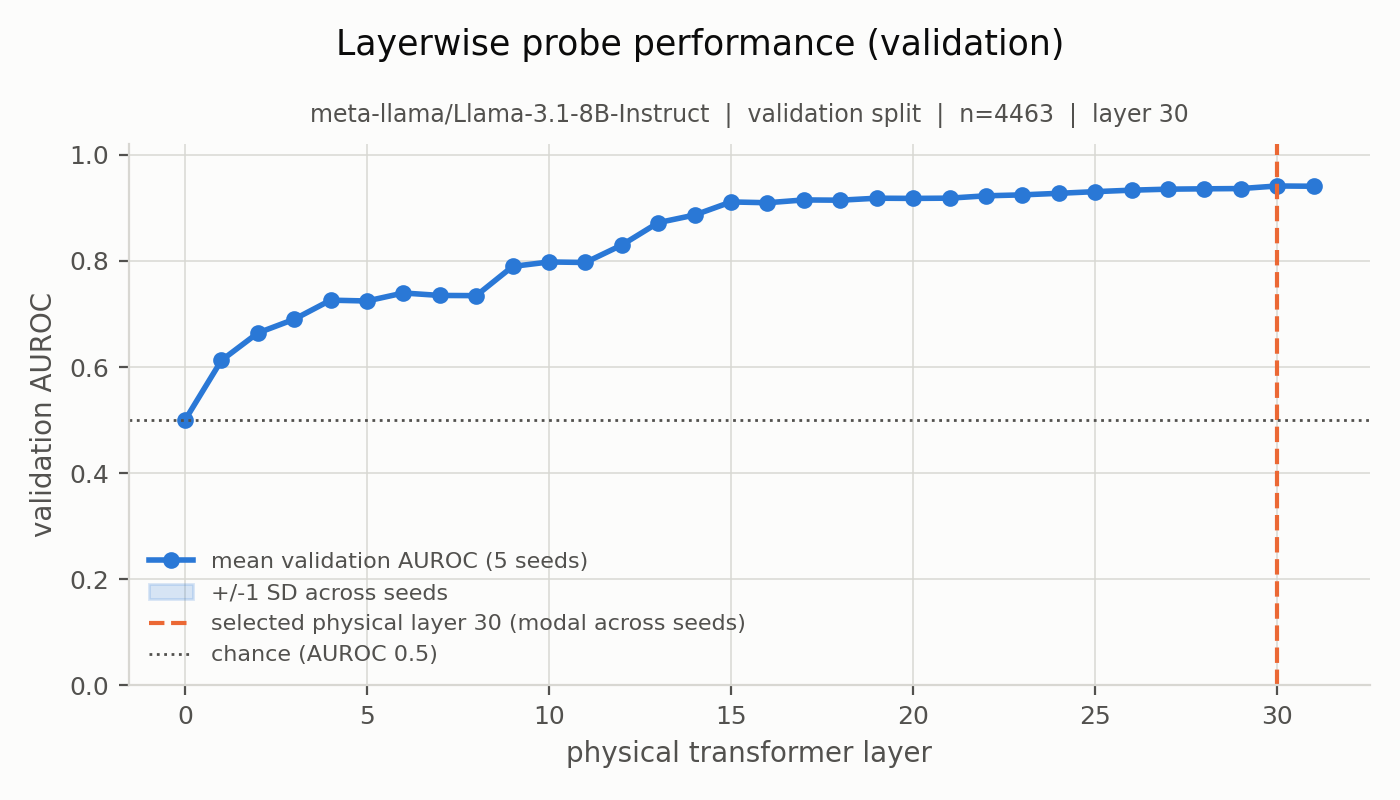
\includegraphics[width=0.49\linewidth]{figures/judge/layerwise_probe.png}
\hfill

\includegraphics[width=0.49\linewidth]{figures/neutral/layerwise_probe.png}
\caption{Layerwise probe performance for the explicit bluff-judgement prompt (left) and question-stripped neutral-state prompt (right). Physical transformer layers are shown on the horizontal axis. Layer selection uses validation AUROC only, with the frozen selection evaluated on the held-out test partition.}
\label{fig:layerwise-probes}
\end{figure}

\begin{table}[t]
\centering
\caption{Strict held-out probe results for the two prompt variants. Layer selection uses validation AUROC only.}
\begin{tabular}{lrrrr}
\toprule
Variant & Selected layer & Val. AUROC & Test AUROC & Prompt-text AUROC \\
\midrule
Explicit judgement & 30 & 0.9413 & 0.9360 & 0.7817 \\
Neutral state & 31 & 0.9402 & 0.9351 & 0.7825 \\
\bottomrule
\end{tabular}
\end{table}

The learning curves show a smooth increase with data. For the explicit judgement variant, mean test AUROC across five group-level subsamples is 0.7624 at 500 groups, 0.8772 at 2,000, 0.9168 at 8,000, 0.9300 at 20,000, and 0.9359 at 31,000. The neutral-state variant follows the same qualitative pattern: 0.7100, 0.8495, 0.9069, 0.9281, and 0.9346 at the corresponding sizes. This scaling behavior suggests that the late-layer signal is not an artifact of one large training condition.

\begin{figure}[t]
\centering
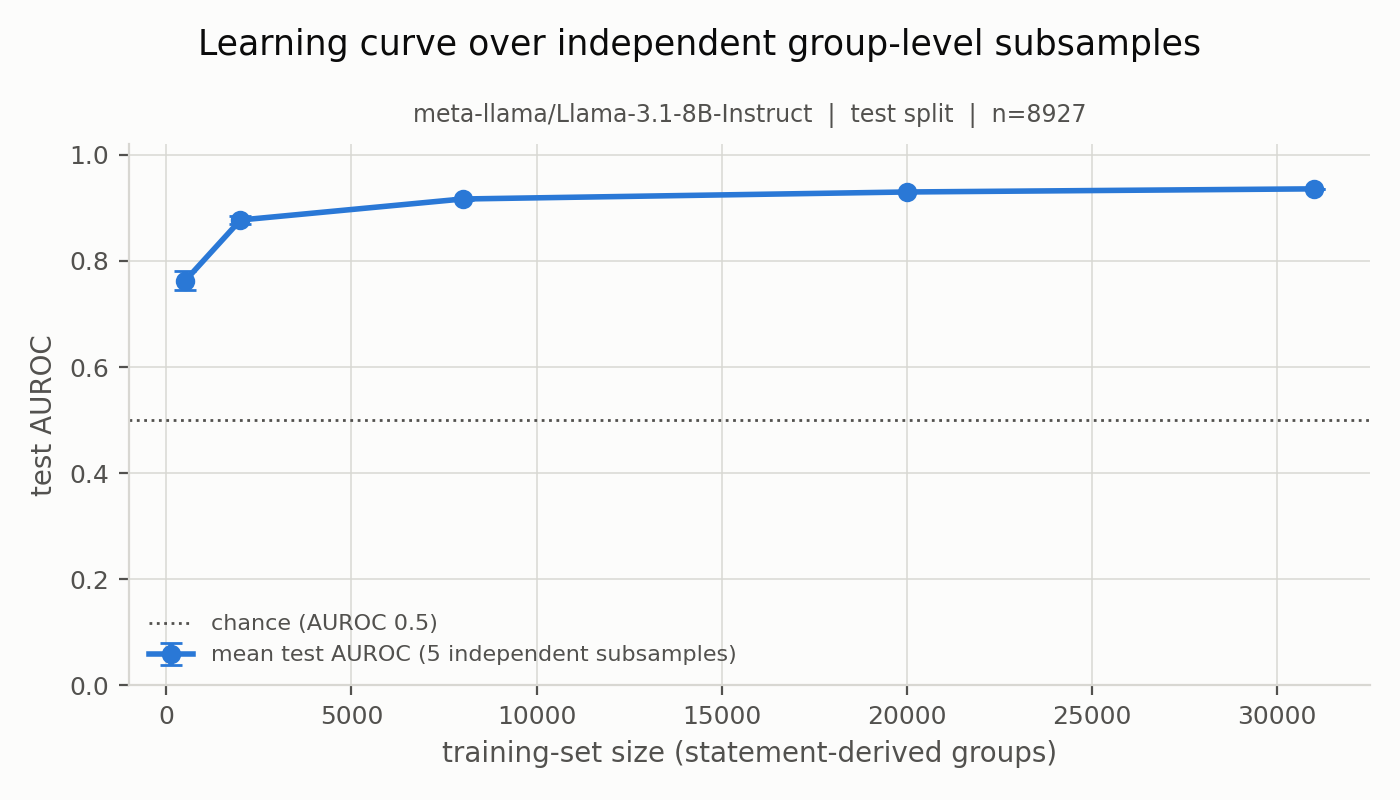
\includegraphics[width=0.49\linewidth]{figures/judge/learning_curve.png}
\hfill

\includegraphics[width=0.49\linewidth]{figures/neutral/learning_curve.png}
\caption{Learning curves for the explicit judgement variant (left) and neutral-state variant (right). Training-set size is measured in statement-derived groups, not verified independent poker hands. Each point summarizes five independent group-level subsamples evaluated on the same frozen test partition.}
\label{fig:learning-curves}
\end{figure}

\subsection{Poker-state variables explain a large fraction of the signal}
The nuisance-only baseline reaches test AUROC 0.9204 and PR-AUC 0.6166, close to the 0.9360 hidden-state probe. This establishes that ordinary poker-state information alone predicts the operational bluff label very strongly.

The primary residualization control strengthens this conclusion. The unadjusted layer-30 hidden-state probe reaches AUROC 0.9360, whereas the residualized probe reaches 0.7220, an absolute drop of 0.2141. Thus, a substantial portion of the linearly accessible bluff-label information overlaps with representations of observed poker-state variables.

Matched-subset analyses show the same pattern from another angle. Test AUROC remains 0.9207 when action-matched, 0.9244 when street-matched, 0.9297 when position-matched, and 0.9251 under the available board matching control. Matching on made-hand category has the largest effect, reducing AUROC to 0.8426. Because every row already contains the same raise action category, action matching is largely satisfied by construction.

The hidden states also make the nuisance variables themselves highly decodable. Street is decoded at 1.000 accuracy, position at approximately 1.000, board texture at 0.914, board pairing at 0.966, and made-hand category at 0.756. Amount faced is predicted with $R^2\approx0.966$. These diagnostics are consistent with the interpretation that the late residual stream contains a rich representation of the poker state from which the bluff label can be inferred.

The appropriate conclusion is therefore not that layer 30 contains a clean deception variable. Rather, the late hidden state contains information predictive of the bluff label, much of which is entangled with ordinary strategic state.

\begin{figure}[t]
\centering
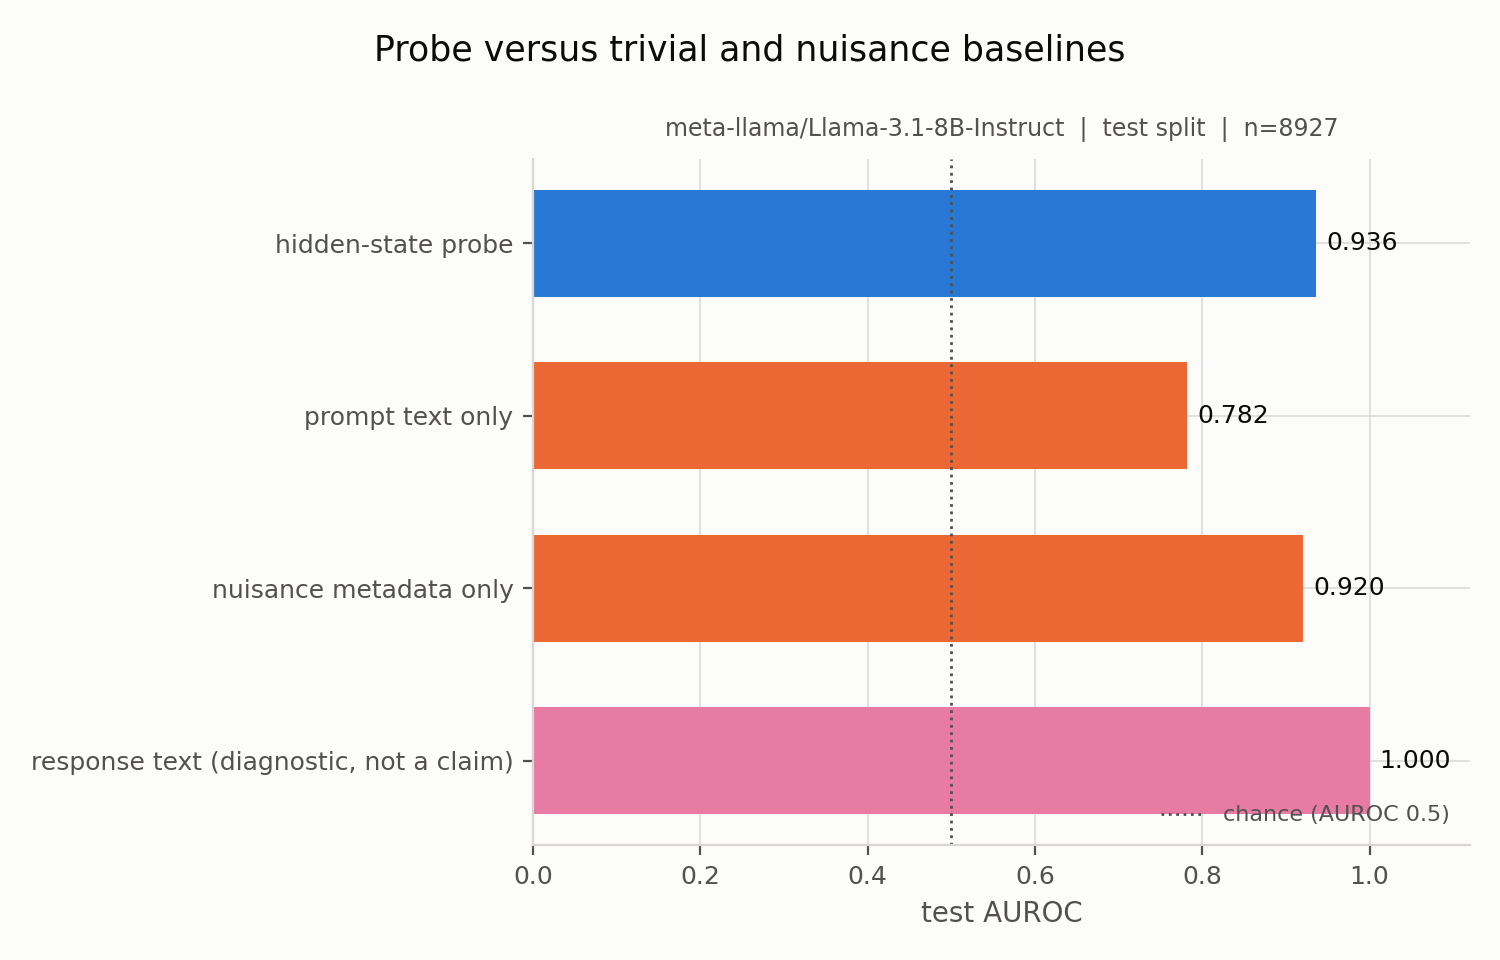
\includegraphics[width=0.49\linewidth]{figures/judge/nuisance_baselines.png}
\hfill
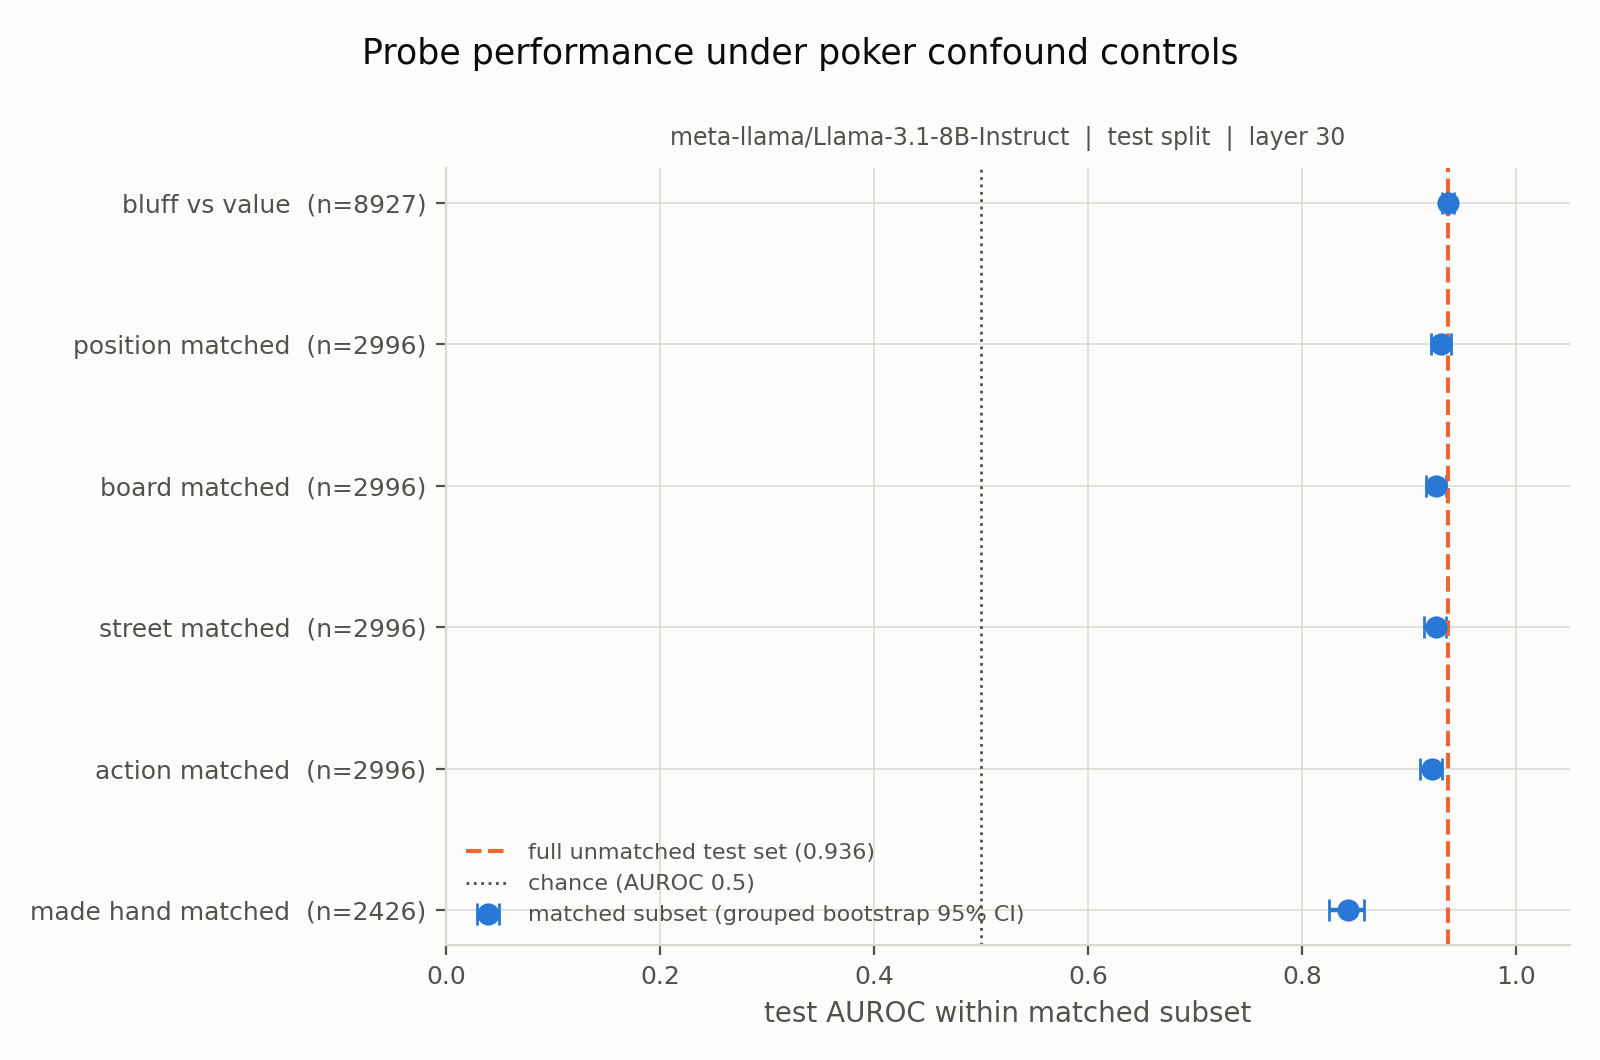
\includegraphics[width=0.49\linewidth]{figures/judge/confound_subsets.png}
\caption{Poker-state confound diagnostics for the explicit judgement variant. Left: the hidden-state probe alongside text and nuisance baselines. Right: matched-subset probe performance under available nuisance controls. Together these results show that ordinary poker-state information accounts for a substantial fraction of the apparent bluff-label signal.}
\label{fig:confounds}
\end{figure}

\subsection{Interventions causally modulate bluff judgement, but specificity is limited}
The forced-choice endpoint is well behaved at baseline: approximately 97.8\% of output probability mass lies on the allowed Yes/No options. Steering along the two orientations of the learned probe direction produces a signed, approximately dose-dependent response. At strength 4, one orientation changes $P(\text{Yes})$ by approximately $-0.019$, while reversing the direction changes it by approximately $+0.018$.

This establishes that the learned direction can causally modulate the model's bluff judgement under the tested intervention. However, the control suite prevents a stronger specificity claim. At the largest tested strength, a matched-norm random direction produces a change of approximately $+0.047$, a shuffled-label direction approximately $+0.027$, and a made-hand nuisance direction approximately $-0.030$. These effects are comparable to or larger than the probe-direction effect. The wrong-token-position control stays near zero, which supports timing specificity, but the overall direction-specificity evidence is weak.

A wrong-layer intervention at strength 4 produces a very large apparent endpoint change, but this condition also collapses valid Yes/No probability mass from roughly 0.98 to 0.04 and chooses the positive option on 99.2\% of prompts. We therefore treat that point as model degradation rather than evidence of stronger causal control. For the intended probe directions and the other non-degenerate controls, valid-choice probability mass remains approximately 0.976 to 0.980.

The intervention result should therefore be described as \emph{causal modulation without demonstrated target specificity}. The probe direction affects the model's bluff judgement, but the present controls do not show that this direction is uniquely associated with bluffing rather than one of several high-impact directions in the local activation geometry.

\begin{figure}[t]
\centering
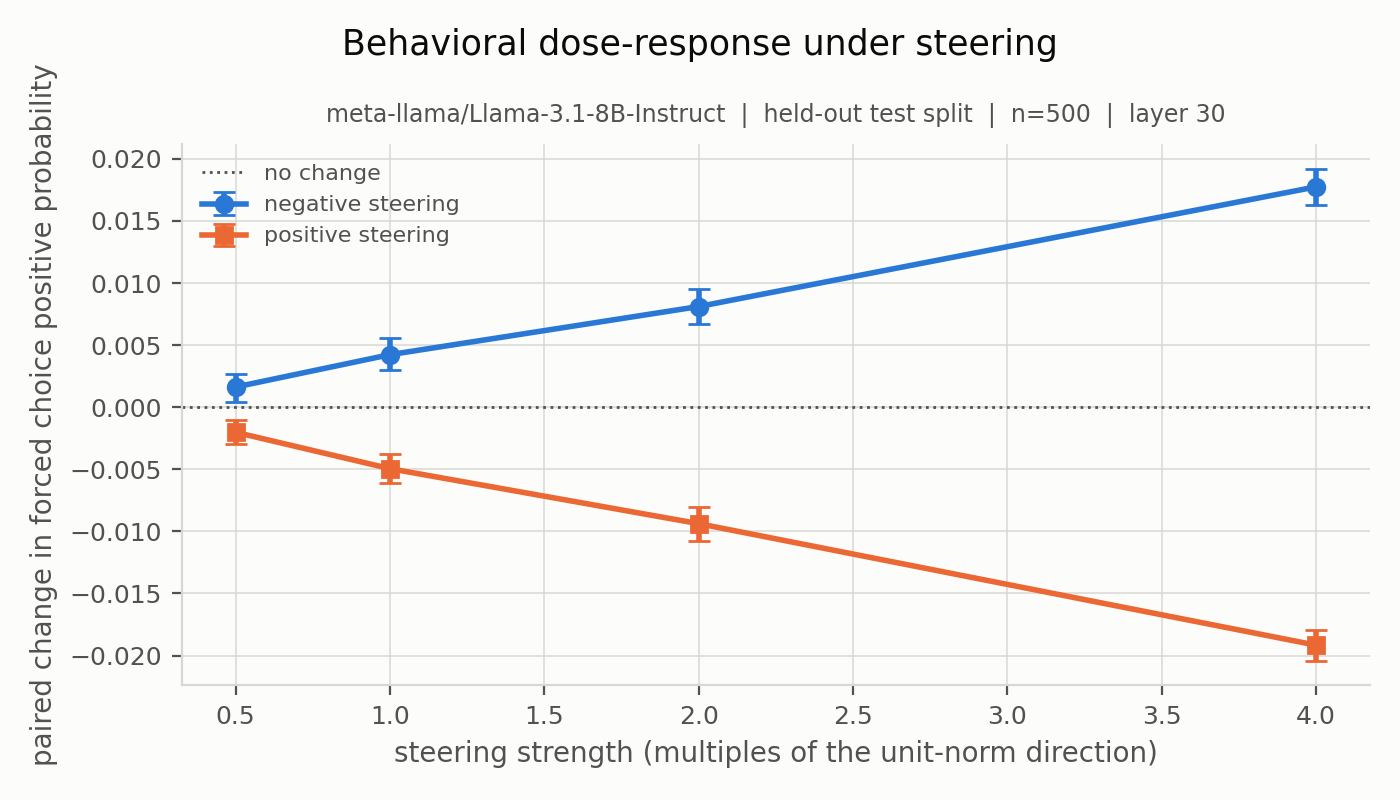
\includegraphics[width=0.49\linewidth]{figures/judge/dose_response.png}
\hfill
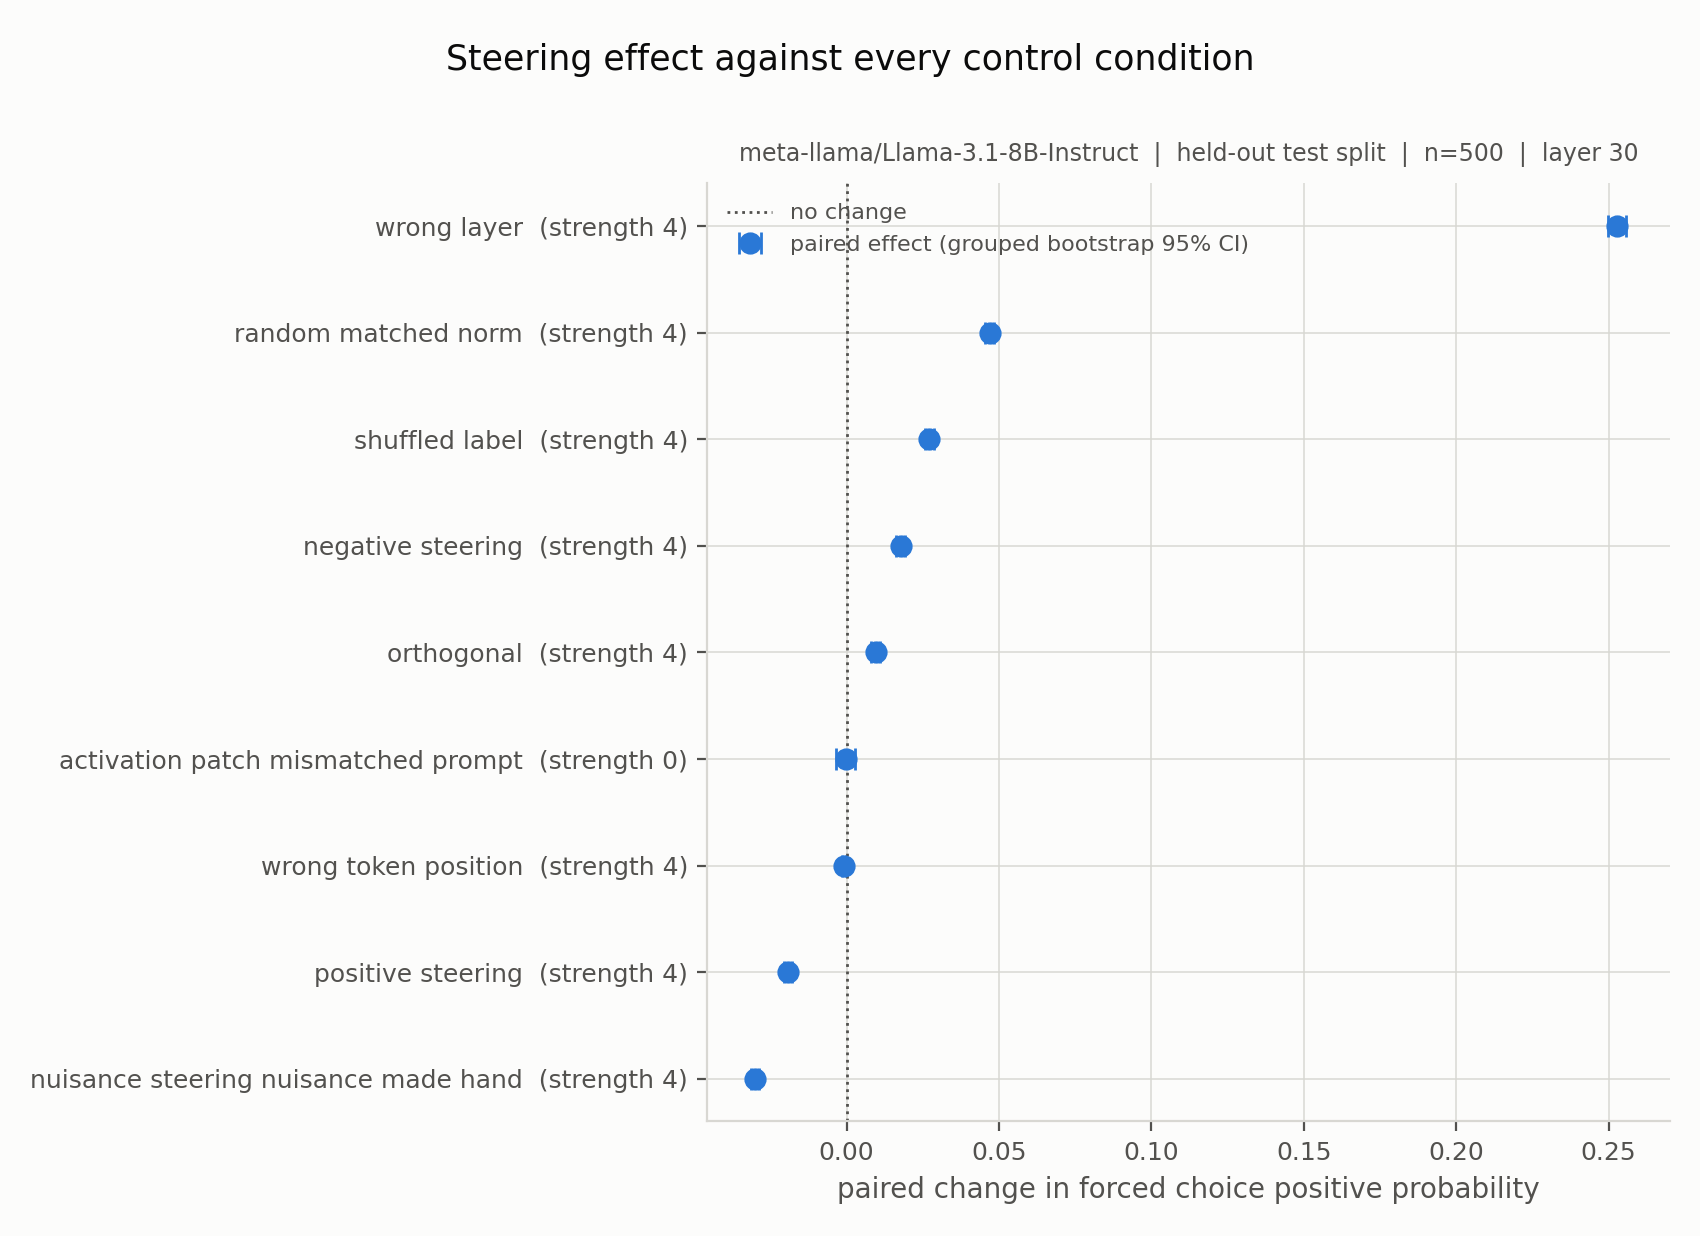
\includegraphics[width=0.49\linewidth]{figures/judge/intervention_controls.png}
\caption{Controlled inference-time interventions on the model's forced-choice bluff judgement. Left: dose response across intervention strengths. Right: comparison with matched control directions. Control effects comparable to the probe-direction effect limit claims of direction specificity.}
\label{fig:interventions}
\end{figure}

\begin{figure}[t]
\centering
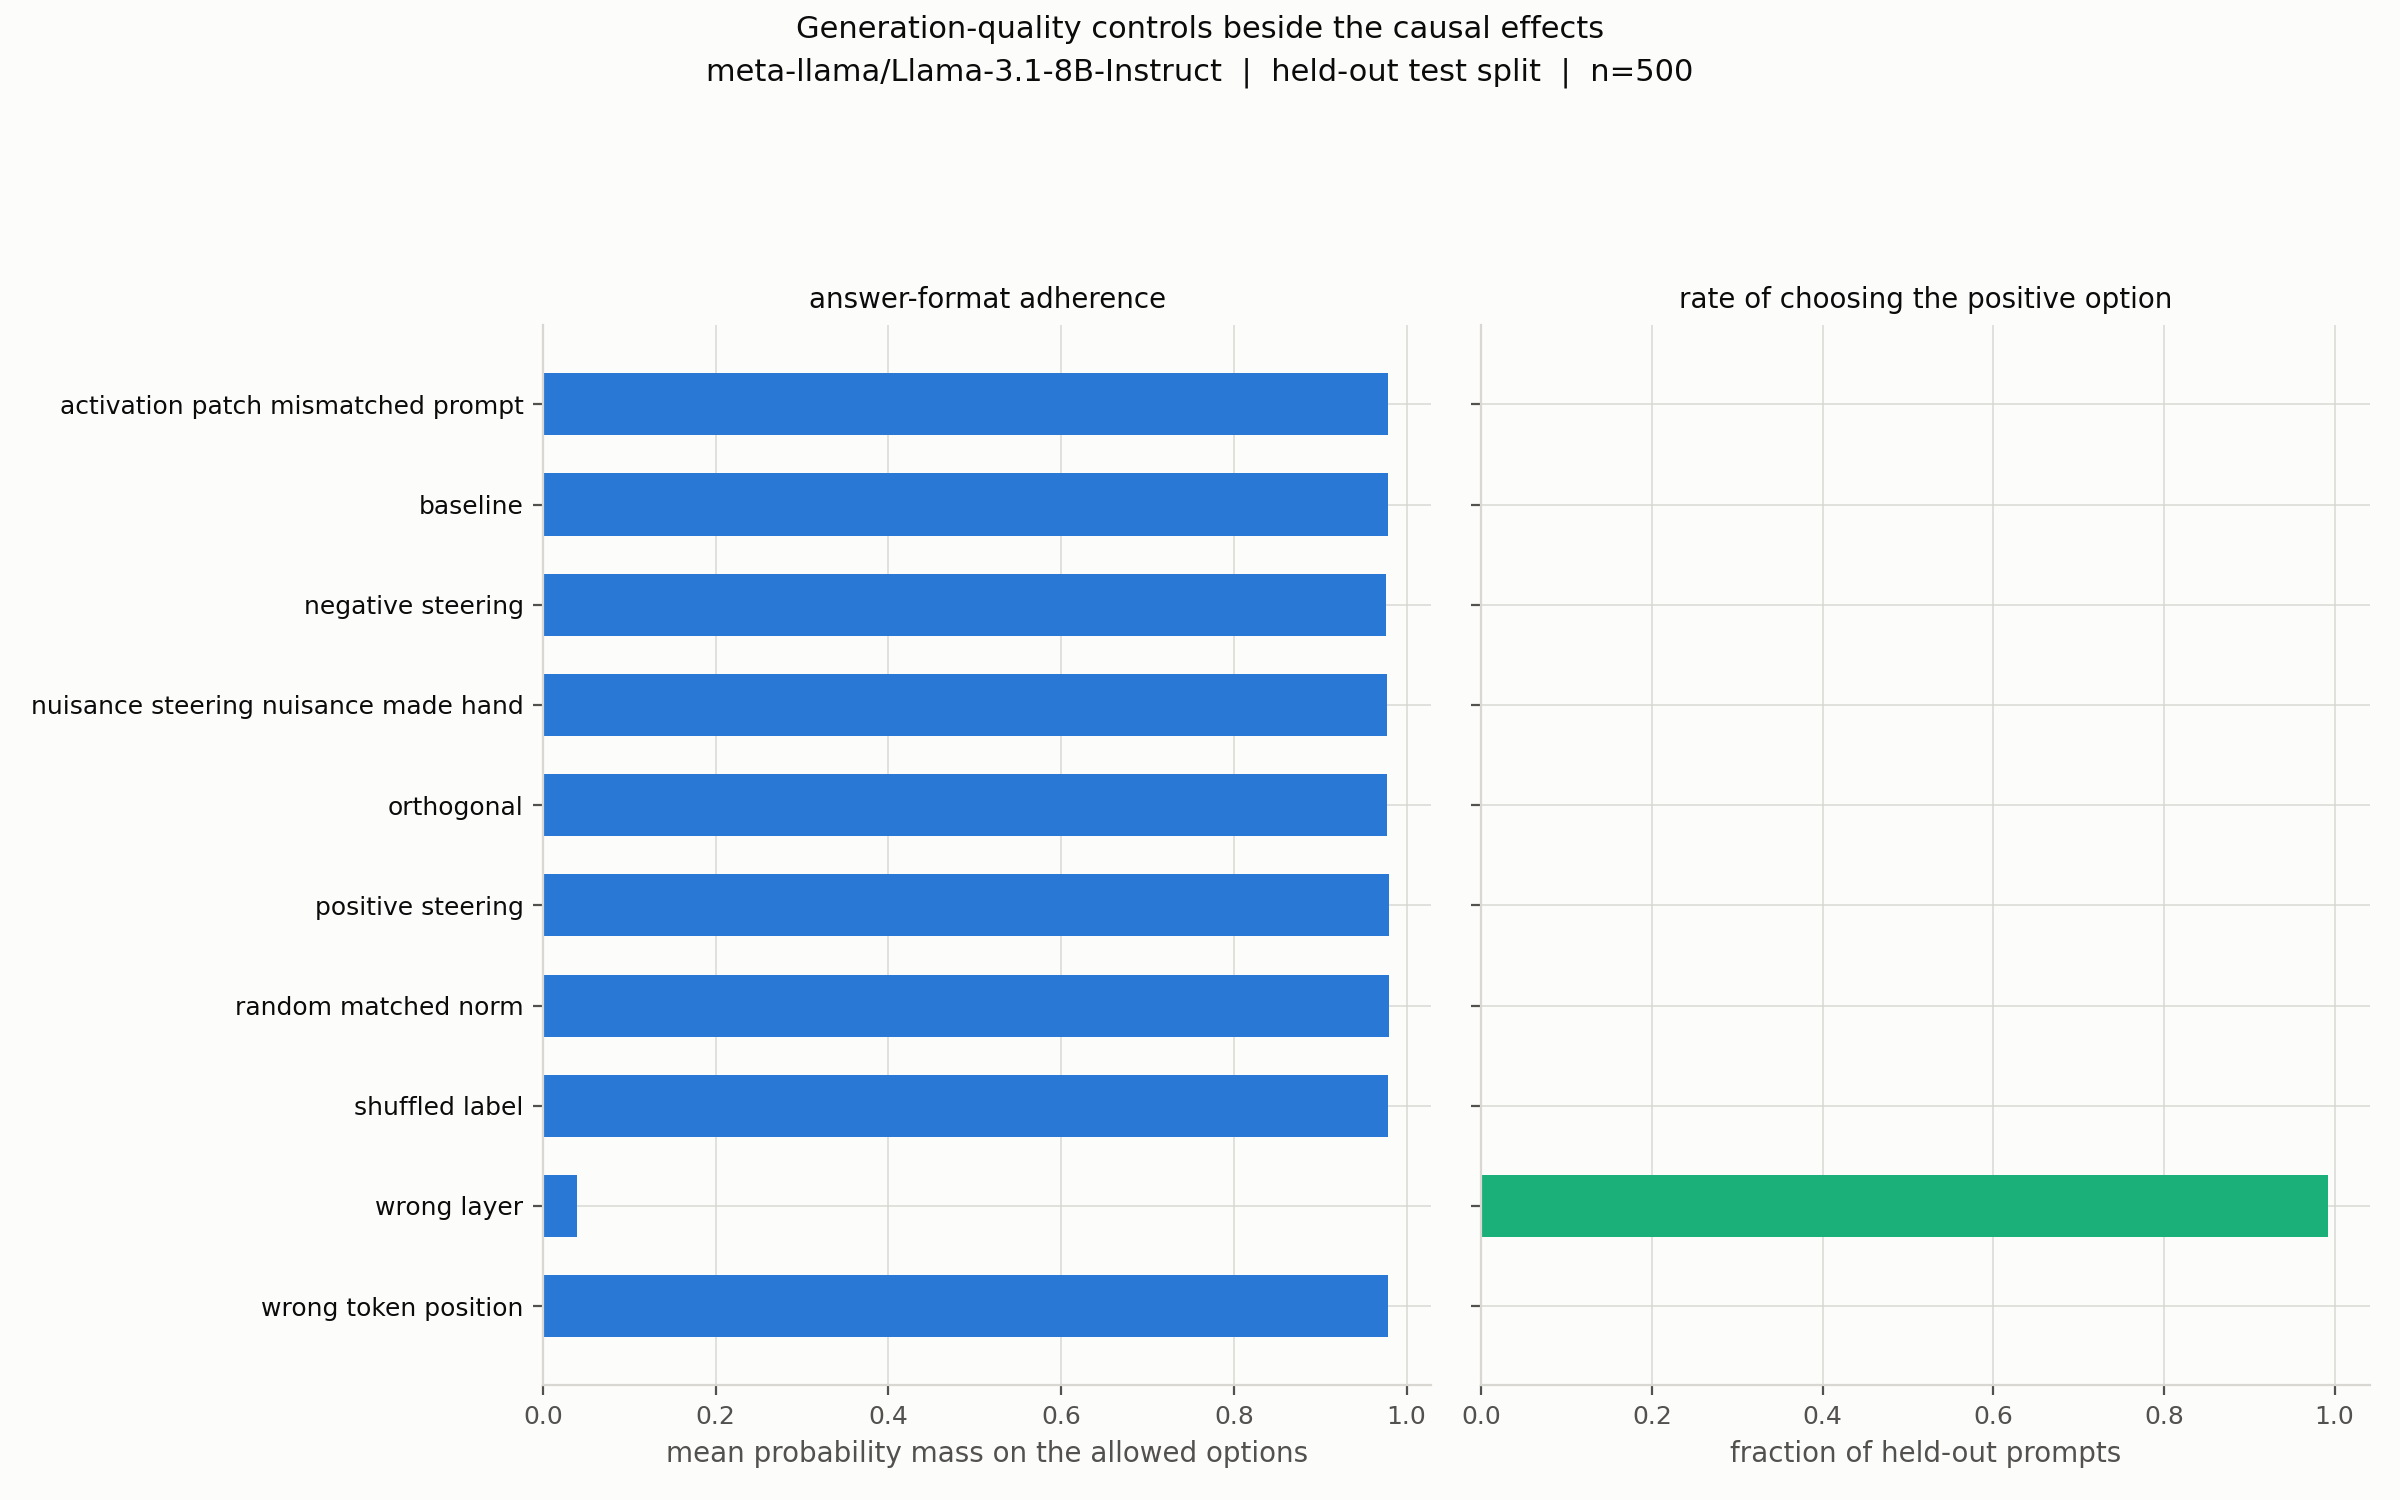
\includegraphics[width=0.72\linewidth]{figures/judge/intervention_quality.png}
\caption{Intervention quality diagnostics. Valid Yes/No probability mass remains high for the intended intervention and most controls, while the strongest wrong-layer intervention is degenerate and is not interpreted as evidence of targeted causal control.}
\label{fig:intervention-quality}
\end{figure}

\subsection{The SAE reconstructs well but does not yield stable bluff features}
The TopK SAE at layer 30 explains 95.17\% of test activation variance while maintaining mean L0 of 64 active features per example, as specified by the TopK architecture. The test dead-feature fraction is 0.756, so most dictionary features do not activate on the test partition.

More importantly for interpretation, dictionary stability across training seeds is low: mean maximum cosine similarity across seed pairs is approximately 0.101. The ten features selected by train-plus-validation bluff-label separability also generalize only modestly to the held-out test set, with single-feature AUROCs roughly spanning 0.42 to 0.59 and a best observed value around 0.593.

These results do not support the earlier interpretation that the SAE exposes stable, interpretable ``deception features.'' They support a narrower statement: a sparse dictionary can reconstruct the selected-layer activation space accurately, but individual coordinates are unstable and weak as standalone bluff-label predictors under the current training setup.

\begin{figure}[t]
\centering
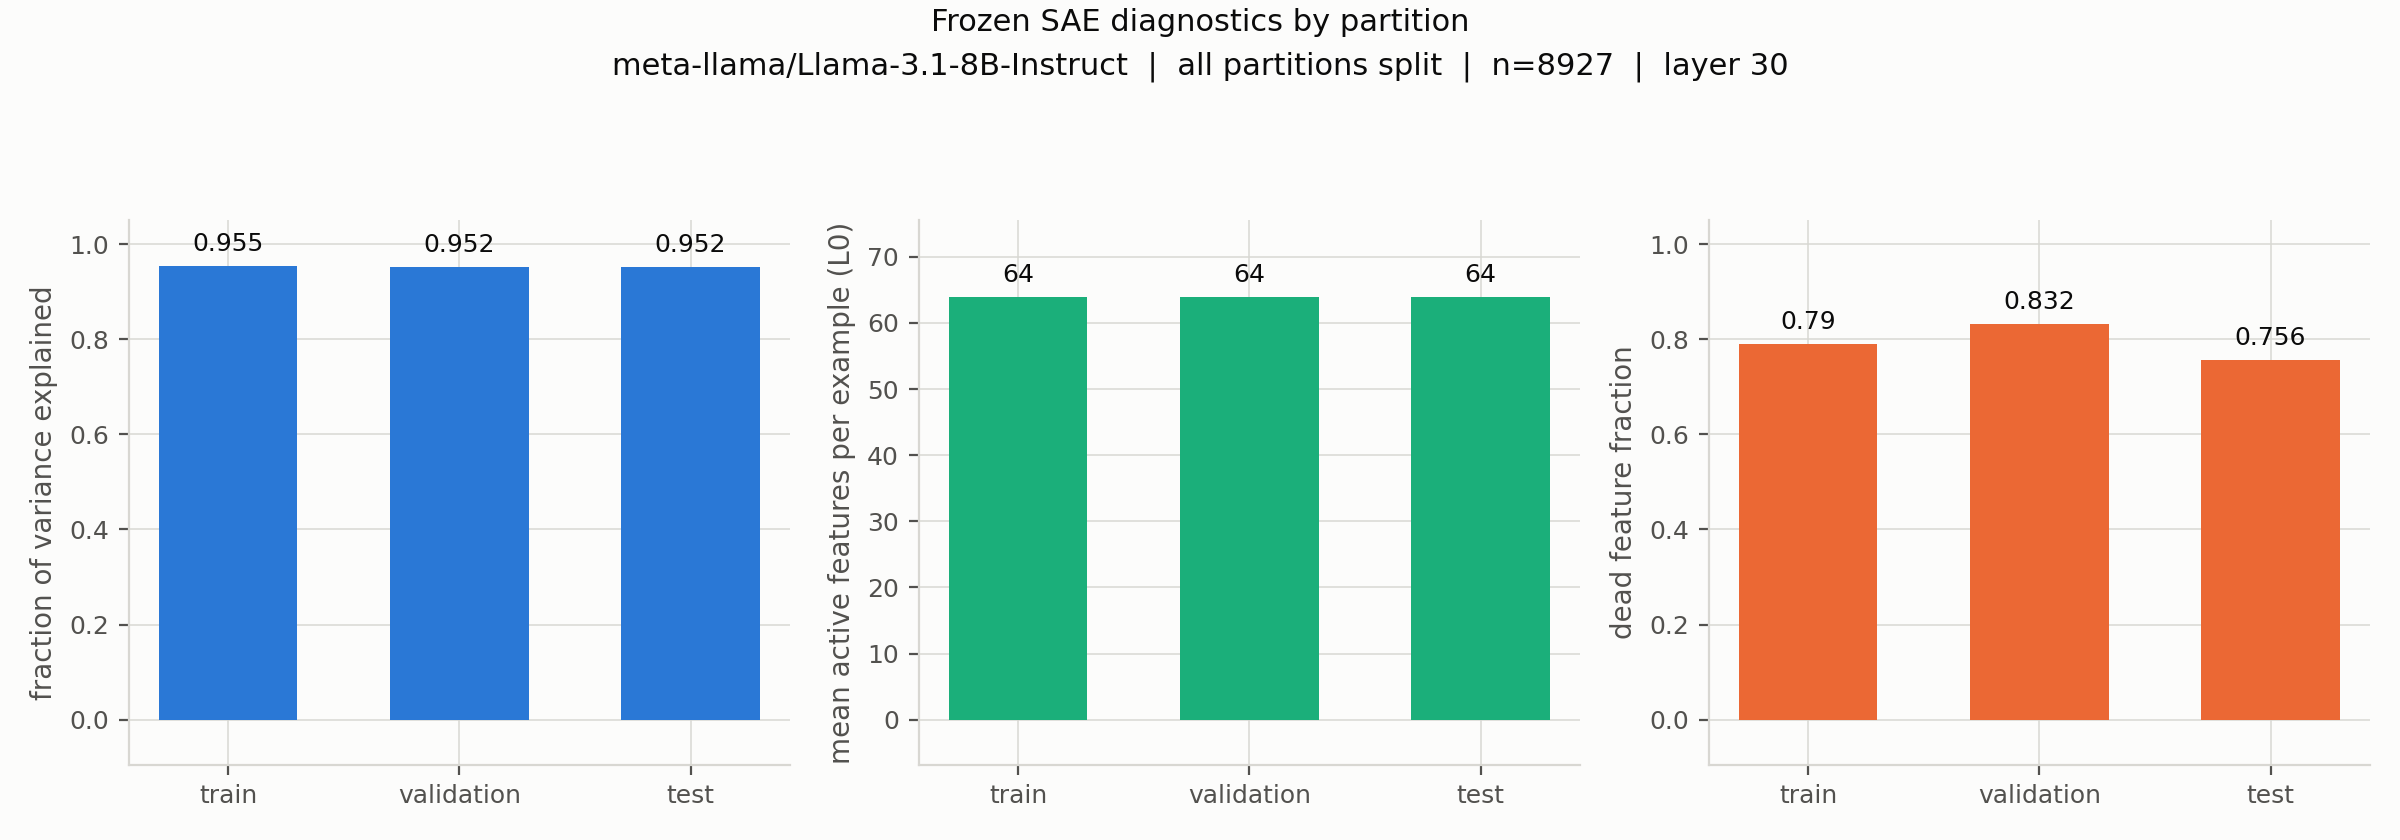
\includegraphics[width=0.49\linewidth]{figures/judge/sae_diagnostics.png}
\hfill
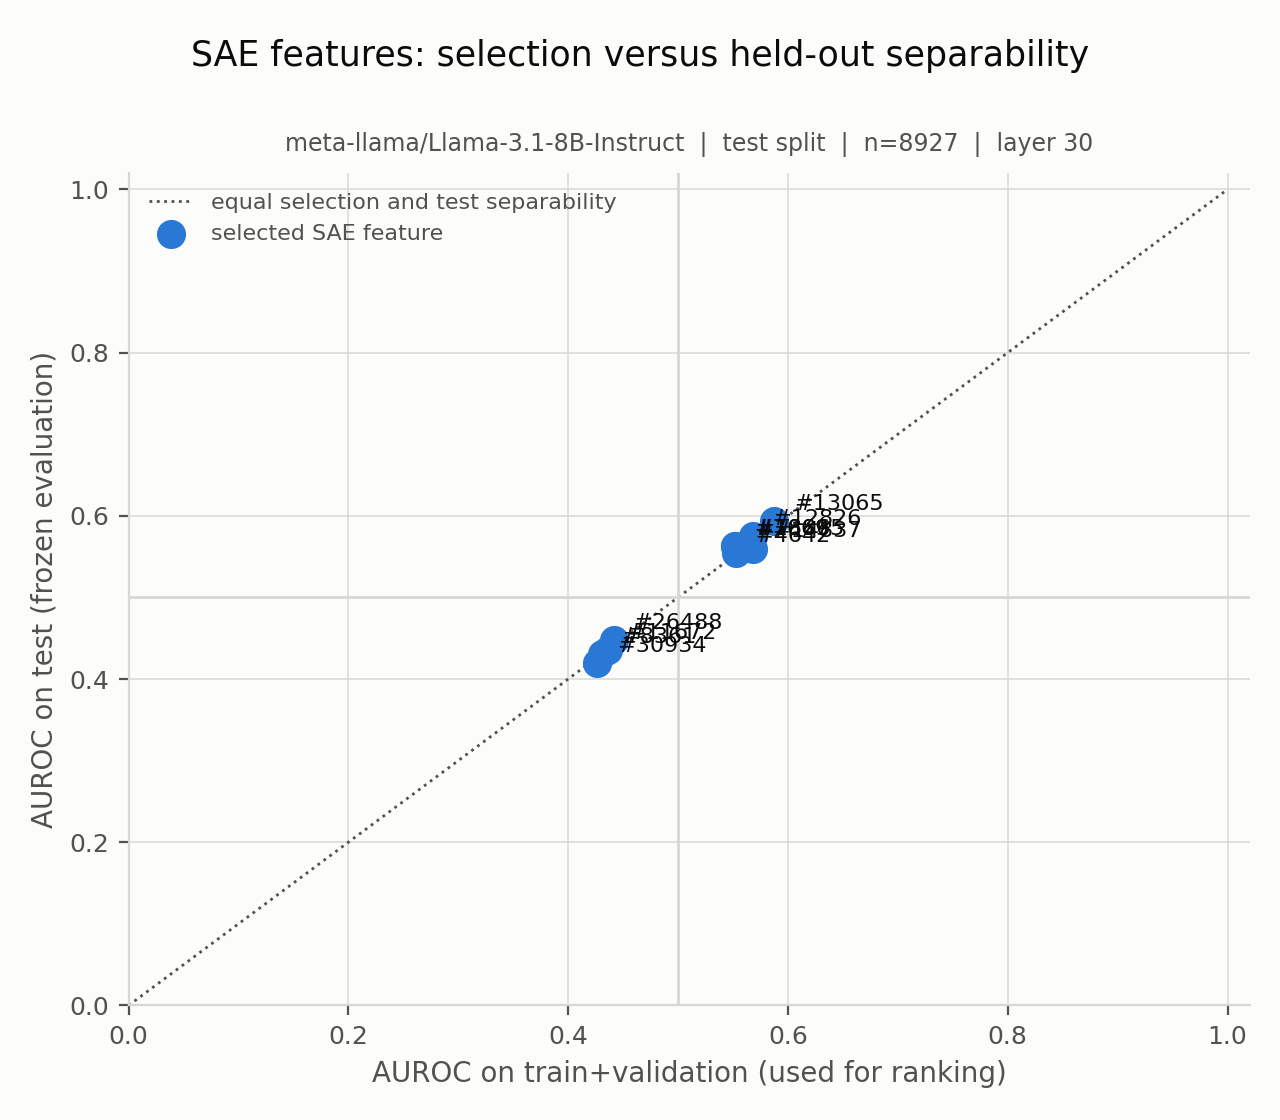
\includegraphics[width=0.49\linewidth]{figures/judge/sae_features.png}
\caption{Sparse-autoencoder results at the selected explicit-judgement layer. Left: reconstruction, sparsity, dead-feature, and stability diagnostics. Right: held-out performance of features selected using training plus validation data. Reconstruction is strong, but individual feature-level bluff associations are modest and unstable.}
\label{fig:sae}
\end{figure}

\section{Discussion}
The most robust finding is not the existence of a single deception direction. It is the coexistence of three facts. First, bluff labels are highly linearly decodable from late Llama-3.1-8B hidden states. Second, the same hidden states strongly encode ordinary poker-state variables that nearly predict the label on their own. Third, interventions along a probe-derived direction can change the model's bluff judgement, but several matched control directions can also produce substantial changes.

The explicit-versus-neutral comparison rules out one simple explanation of the probe result. The late-layer signal persists almost unchanged after removing the explicit bluff question, so it is not merely a representation of the instruction ``classify this as a bluff.'' The confound controls reveal a different and more substantive explanation: the label is deeply entangled with game state. A model that represents hand strength, position, street, board structure, and bet size can become highly predictive of a bluff label without representing deception as a distinct mechanistic variable.

This distinction matters for how activation probes are interpreted. A probe can reveal that a label is accessible from an activation without establishing why it is accessible. In a structured domain, nuisance variables may carry most of the relevant information. We therefore view the residualized AUROC of 0.722, the made-hand-matched AUROC of 0.843, and the 0.920 nuisance-only baseline as at least as important as the raw 0.936 headline probe.

The intervention experiment provides stronger evidence than a stored-vector probe-score perturbation because the intervention occurs inside the live model and the primary endpoint is the model's own output distribution. Even so, causal change is not the same as causal specificity. The matched controls show that several directions can move the forced-choice endpoint. This limits any claim that the probe direction isolates a unique bluff mechanism. A stronger result would require a larger separation between the target direction and controls, replication across models or independent poker tasks, and preferably a task in which the subject model itself chooses an action rather than judges someone else's action.

The SAE result offers a parallel caution. Strong reconstruction quality does not imply semantic interpretability. The low cross-seed dictionary stability and modest held-out single-feature AUROCs argue against assigning strong semantic names to individual features. The sparse representation is useful as an alternate coordinate system, but the current evidence does not establish monosemantic bluff features.

Taken together, these results support a methodological lesson for mechanistic studies of strategic concepts. Decodability, nuisance-controlled residual information, intervention sensitivity, intervention specificity, and sparse-feature stability are distinct levels of evidence. Treating them separately produces a more conservative but more reproducible account of what the activations actually support.

\section{Limitations}
The labels are GPT-4o judgements rather than human or solver adjudications, so label validity is inherited from the labelling model and prompt. A future benchmark should include independently adjudicated examples, especially ambiguous draws and semi-bluffs.

Dataset lineage is incomplete. PokerBench is recoverable as the source dataset, but the exact source split and revision, original hand/session identifiers, final selection script, upstream action-generation procedure, and exact GPT-4o snapshot are unavailable. Statement-derived grouping protects against direct statement duplication across partitions but does not prove independence across underlying dealt hands or trajectories.

The available metadata does not support true equity matching or a reliable pot-size control. The present residualization therefore cannot remove every strategically relevant variable. In addition, exact duplicates remain in the source dataset, although group-safe splitting prevents identical statement-derived groups from crossing partitions.

The strict real-run experiments reported here use one subject model, Llama-3.1-8B-Instruct, and one poker scenario. Historical Mistral and Qwen runs are not used as strict cross-architecture evidence because they were not repeated under the final protocol. Likewise, cross-context transfer cannot be evaluated with only one real scenario.

The causal endpoint measures the model's judgement of an observed raise. The subject model is not choosing whether to bluff, so the intervention does not demonstrate increased or decreased deceptive behavior. The strongest supported claim is that interventions change the model's forced-choice bluff judgement under the tested conditions.

Finally, the SAE exhibits substantial dead features and low seed stability. Feature-level interpretations should therefore be treated as exploratory until they are replicated across dictionaries, validated with targeted examples, and tested with feature-level causal interventions.

\section{Related Work}
Linear probes and affine readouts are widely used to study information accessible in language-model activations \citep{burns2022,belrose2023}. Such methods establish linear decodability but do not by themselves identify the source, specificity, or causal role of the decoded information. Our confound controls are motivated by this distinction.

Sparse autoencoders provide a complementary approach for decomposing dense activations into sparse feature dictionaries \citep{cunningham2023}. We adopt a TopK formulation and emphasize reconstruction, sparsity, dead-feature rate, held-out feature evaluation, and cross-seed stability rather than inferring semantic meaning from a small number of highly associated examples.

Activation steering and inference-time intervention have been used to test whether directions in activation space can influence model outputs \citep{li2023,turner2023}. Our intervention design follows the same broad idea but evaluates a probe-derived direction against matched random, orthogonal, shuffled-label, wrong-layer, wrong-token, mismatched-prompt patching, and nuisance-direction controls. This makes the distinction between causal modulation and direction specificity explicit.

More broadly, mechanistic-interpretability work emphasizes causal testing of internal representations rather than relying only on correlational readouts \citep{elhage2021,geiger2021}. Our results illustrate why this standard is particularly important for strategic labels that are predictable from ordinary task semantics.

\section{Conclusion}
We find that an operational poker bluff label is strongly decodable from late Llama-3.1-8B hidden states under a strict pre-response probing protocol. The result persists when the explicit bluff question is removed, but poker-state variables alone nearly match the raw probe and nuisance residualization substantially reduces performance. Inference-time steering along the learned probe direction changes the model's forced-choice bluff judgement in a signed dose-dependent way, yet several control directions also produce substantial effects, preventing a claim of a uniquely identified bluff mechanism. An unsupervised sparse autoencoder reconstructs the selected activation space well but does not yield stable, strongly label-predictive individual features.

The resulting picture is more constrained than a ``deception circuit'' claim but more informative. Late activations carry robust information about the operational bluff label, that information is strongly entangled with ordinary poker strategy, and causal sensitivity alone is insufficient to establish mechanism specificity. Future work should use independently adjudicated labels, verified hand identities, multiple strategic contexts, additional subject models, and model-as-actor tasks in which the intervention can be evaluated against actual strategic choices.

\section*{Impact Statement}
Internal monitoring of strategic behavior is relevant to model oversight, but probe accuracy can be misleading when labels correlate with ordinary task variables. Our results therefore argue for caution in deploying activation probes as deception detectors without strong nuisance controls, held-out validation, and causal specificity tests. The same intervention methods could in principle be used to manipulate model judgements, so we emphasize transparent evaluation and defensive interpretability rather than optimization toward deceptive behavior.

\appendix
\section{Additional Experimental Details}
\subsection{Dataset and split statistics}
The dataset contains 44,631 rows and 44,311 statement-derived groups. The frozen strict split contains 31,241 training rows, 4,463 validation rows, and 8,927 test rows. The positive bluff-label rate is 16.8\%. Group identifiers are derived from statement content and must not be interpreted as verified independent poker hands.

\subsection{Prompt variants}
The explicit variant retains the bluff-judgement question and extracts the final prompt-token state immediately before answer generation. The neutral variant removes the target question and ends at the observed action description. Both use the same subject model revision and the same split.

\subsection{Probe learning curves}
For the explicit judgement variant, mean test AUROC over five independent group-level subsamples is 0.7624, 0.8772, 0.9168, 0.9300, and 0.9359 for 500, 2,000, 8,000, 20,000, and 31,000 groups, respectively. For the neutral-state variant the corresponding values are 0.7100, 0.8495, 0.9069, 0.9281, and 0.9346.

\subsection{Causal quality controls}
Baseline valid-choice mass is approximately 0.978. Across intended positive and negative steering, orthogonal steering, random matched-norm steering, shuffled-label steering, nuisance steering, wrong-token-position steering, and mismatched-prompt patching, mean valid-choice mass remains near 0.976 to 0.980. The principal quality failure is the wrong-layer intervention at strength 4, where mean valid-choice mass falls to approximately 0.040 and the positive-choice rate rises to 0.992. We exclude this degenerate high-strength point from any specificity interpretation.

\subsection{SAE diagnostics}
The primary SAE uses 32,768 TopK features with $k=64$. On test it explains 0.9517 of activation variance, has mean L0 approximately 64, and a dead-feature fraction of 0.7558. Cross-seed dictionary stability, measured by mean maximum cosine similarity across seed pairs, is approximately 0.1009. The ten features selected on train plus validation achieve held-out single-feature AUROCs ranging from approximately 0.42 to 0.59.

\section{Reproducibility and Artifact Traceability}
Every strict run records the dataset checksum, split manifest, model revision, tokenizer revision, activation-layer mapping, prompt hashes, artifact hashes, and environment metadata. Figure generation consumes only real result artifacts, writes a source-data CSV for each figure, and records source-artifact checksums in a figure manifest. The strict audit passes for both the explicit judgement and neutral-state real runs. Controls that require unavailable metadata are represented explicitly as \texttt{not\_run} with a reason rather than silently omitted or approximated.

% Publication figures above are generated from the strict real-run artifacts.
% Their source CSVs and figure manifests are stored alongside the PNG files.
